\section{Methods}\label{sec:2}

\subsection{Design}\label{sec:2.1}

The object measured is the authorising provision. An authorising provision is a paragraph of a legal instrument that grants, conditions or withdraws a permission, and is not a penalty provision. The corpus contains 1,014 of them. For each, the study decides one predicate: does this provision carry a determinate operator and reach a named technical evaluation through the cross-references written in the law?

Nothing in that predicate requires the analyst to choose which propositions to test, which is where the previous design of this study was weakest. Two analyst-dependent steps remain and are handled differently. The vocabulary that identifies authorisations, evaluations and operators is fixed once and then validated against a language-stratified sample (Section 2.6). The mission analysis that decides which regulatory domains are in scope is documented and its output published, but it enters the measurement only through the scope restriction, whose effect is reported as a sensitivity (Section 3.7).

\subsection{Missions and the domains they place in scope}\label{sec:2.2}

The two police-robot missions were analysed with System-Theoretic Process Analysis following the sequence of Leveson and Thomas \citep{LevesonThomas2018STPA}: losses, hazards, control structure, unsafe control actions under four guidewords, safety constraints, and the lossscenario step that yields causal constraints. Mission G is ground-robot sampling at a chemical, biological, radiological or nuclear scene under an incident commander. Mission A is a police small unmanned aircraft searching over an urban area, flyable either under the civil rules or as a public aircraft operation.

The Mission G control structure separates three functions that are often conflated. The sensing subsystem measures and does not classify; the analyst produces the analytical result and may advise the applicable criterion; the incident commander determines whether contamination is present against criteria fixed in advance by standing operating procedure. The commander's determination is by design determinate, and it rests on a measurement. Whether law conditions anything on the validity of that measurement is the question the rest of the paper measures (Fig. 1a).

The analysis produced 63 constraints: 44 safety constraints, 12 causal constraints and 7 accountability elements drawn from Bovens's framework \citep{Bovens2007Accountability} extended with three conditions that Metcalf et al. identify as necessary if an impact assessment is to constitute an accountability relationship \citep{Metcalf2021AIA}. The registers are published in full and are summarised here rather than tabulated, because they do two jobs in this paper and neither is arithmetic. They fix which regulatory domains apply, and therefore which sixteen instruments enter the corpus, which is the only sense in which the measurement depends on them; Section 3.8 reports the reliability test that led us to withdraw constraint-level counts. And they supply the one place where the analysis speaks back to the result: two of the twelve causal constraints concern whether the competence of the person operating the robot is demonstrated against the conditions the mission presents, and the most completely specified certification scheme in the

ground corpus turns out to contain no operator requirement at all (Section 4.4). A reader who wants the measurement without the control analysis can take the sixteen instruments as given and lose nothing except that observation.

\subsection{The audited corpus}\label{sec:2.3}

Sixteen instruments were admitted, on three conditions: official machine-readable text, coverage of both the platform-regulating and the conduct-regulating side, and inclusion of the domains in which a binding of the required kind is known to exist.

Three exclusion classes were fixed before adjudication. Non-normative material (foresight reports, recommendations, guidance) was excluded because it cannot supply a determinate authorisation outcome; FAA AC 00-1.1B is retained not as a source of bindings but as the documentary basis for the United States carve-out rule. Boilerplate (entry into force, addressees, repeal, transitional provisions, Korean penalty and administrative-fine articles, Japanese penalty and supplementary provisions) was excluded by pattern, together with the paragraphs contained within it. That exclusion did not originally execute for the Japanese statute and we report the defect and its repair. The extractor keyed Japanese articles by number alone, and the Act carries 355 articles in its main body and 221 in its supplementary provisions, carrying 42 distinct numbers of which 34 collide with the main body; the later occurrence overwrote the earlier, so 52 of the 1011 main-body paragraph nodes held supplementary text instead of their own, and 26 supplementary paragraphs entered as nodes the main body does not have. No paragraph was deleted: a last-wins dictionary replaces a key's contents and does not remove the key. An earlier version of this passage reported thirty-six replacements and eighty-one losses; neither figure is reproducible from the mechanism just described, and a released script, \texttt{verify/manuscript\\texttt{\_derived}.py}, now recomputes all of these from the corpus on every run. The extractor now stops at the first supplementary-provision element. The repair removes 4 provisions from the returned set, all of which the audit of Section 2.7 had already rejected as deeming rules of the form a person deemed under Supplementary Provision Article N to have passed, and it introduces no provision that the audit has not seen. Audited bindings are unchanged. The effect on the reported totals is 1,016 authorising provisions to 1,006 and 78 returned provisions to 74, before the two corrections reported in Section 2.10 take the figures to 1,003 and 77, and before the extraction repairs of Section 2.10 take them to 1,019 and 82. Separately, penalty provisions are also barred from starting a path, because a sanction attached to a breach is not an authorisation conditioned on an evaluation. One instrument could not be admitted for a technical reason: the Korean ministerial notice setting the outdoor mobile robot certification criteria is published as a proprietary wordprocessor file, so it is read and used descriptively in Section 4.4 but contributes no node, edge or count. The Korean Measurement Act could not be retrieved in machine-readable form during the study period and is recorded as not collected.

A further two instruments were added after the rules were frozen, because they are the instruments most likely to refute the paper. Directive 2014/32/EU is the European legal-metrology regime, which exists entirely to condition the marketing of measuring instruments on their metrological performance. 14 CFR Part 89 ties the operation of a standard remote identification unmanned aircraft to equipment produced under an FAA-accepted declaration of compliance, which is a technical requirement on the machine and the nearest thing in the US corpus to the structure we are looking for. Both instruments are reported in full below, neither was excluded on any ground, and both fail the audit: their tier distributions and the reasons are in Sections 3.4 and 3.5.

\begin{table}[!htb]
\centering
\caption{The audited corpus. Every file is pinned by SHA-256 in the supplementary manifest. ``Nodes'' is the number of provision nodes produced; ``Auth.'' the number of authorising provisions; ``T2'' the number the frozen predicate returns, before the audit of Section 2.7. Returned provisions are not bindings: 41 of the 91 survive the audit, and the perinstrument audited counts are given in Table 9 by domain.}
\label{tab:t1}
\footnotesize
\begin{tabularx}{\textwidth}{@{}lrXrrr@{}}
\toprule
Code & Domain & Instrument & Nodes & Auth. & Returned \\
\midrule
EU1139 & aviation & Regulation (EU) 2018/1139, consol. 2 Aug 2026 \citep{EUReg2018_1139} & 682 & 109 & 32 \\
EU947 & aviation & Impl. Regulation (EU) 2019/947, consol. 1 May 2025 \citep{EUReg2019_947} & 133 & 40 & 3 \\
EU945 & aviation & Del. Regulation (EU) 2019/945, consol. 24 Jun 2025 \citep{EUReg2019_945} & 232 & 37 & 1 \\
US107 & aviation & 14 CFR Part 107, small unmanned aircraft \citep{USCFR107} & 220 & 33 & 12 \\
US89 & aviation & 14 CFR Part 89, remote identification \citep{USCFR89} & 136 & 17 & 6 \\
USAC & aviation & FAA AC 00-1.1B, public aircraft operations \citep{FAAAC0011B} & 67 & 5 & 0 \\
JP-RTA & ground & Road Traffic Act, Act No. 105 of 1960 \citep{JPRoadTrafficAct} & 1,366 & 338 & 20 \\
KR-RTA & ground & Road Traffic Act \citep{ROKRoadTrafficAct} & 705 & 110 & 8 \\
KR-RTA-R & ground & Road Traffic Act Enforcement Rule \citep{ROKRoadTrafficEnforcementRule} & 687 & 126 & 3 \\
KR-IRA & ground & Intelligent Robots Act \citep{ROKIntelligentRobotsAct} & 155 & 22 & 3 \\
KR-IRA-D & ground & Intelligent Robots Act Decree \citep{ROKIntelligentRobotsDecree} & 120 & 8 & 0 \\
EUAI & crosscut & Regulation (EU) 2024/1689, AI Act \citep{EUAIAct2024} & 700 & 105 & 2 \\
MID & crosscut & Directive 2014/32/EU, measuring instruments \citep{EUMID2014} & 247 & 34 & 1 \\
LED & crosscut & Directive (EU) 2016/680, law enforcement data \citep{EULED2016} & 250 & 14 & 0 \\
SMC1418 & crosscut & Seattle Municipal Code ch. 14.18 \citep{SeattleMC1418} & 34 & 9 & 0 \\
CAGOV & crosscut & California Government Code \S{}\S{} 7070--7075 \citep{CalGovAB481} & 24 & 7 & 0 \\
\multicolumn{3}{@{}l}{Total: 16 instruments, 21 files, 14,276,114 bytes} & 5,758 & 1,014 & 91 \\
\bottomrule
\end{tabularx}
\end{table}

\begin{figure*}[!t]
\centering
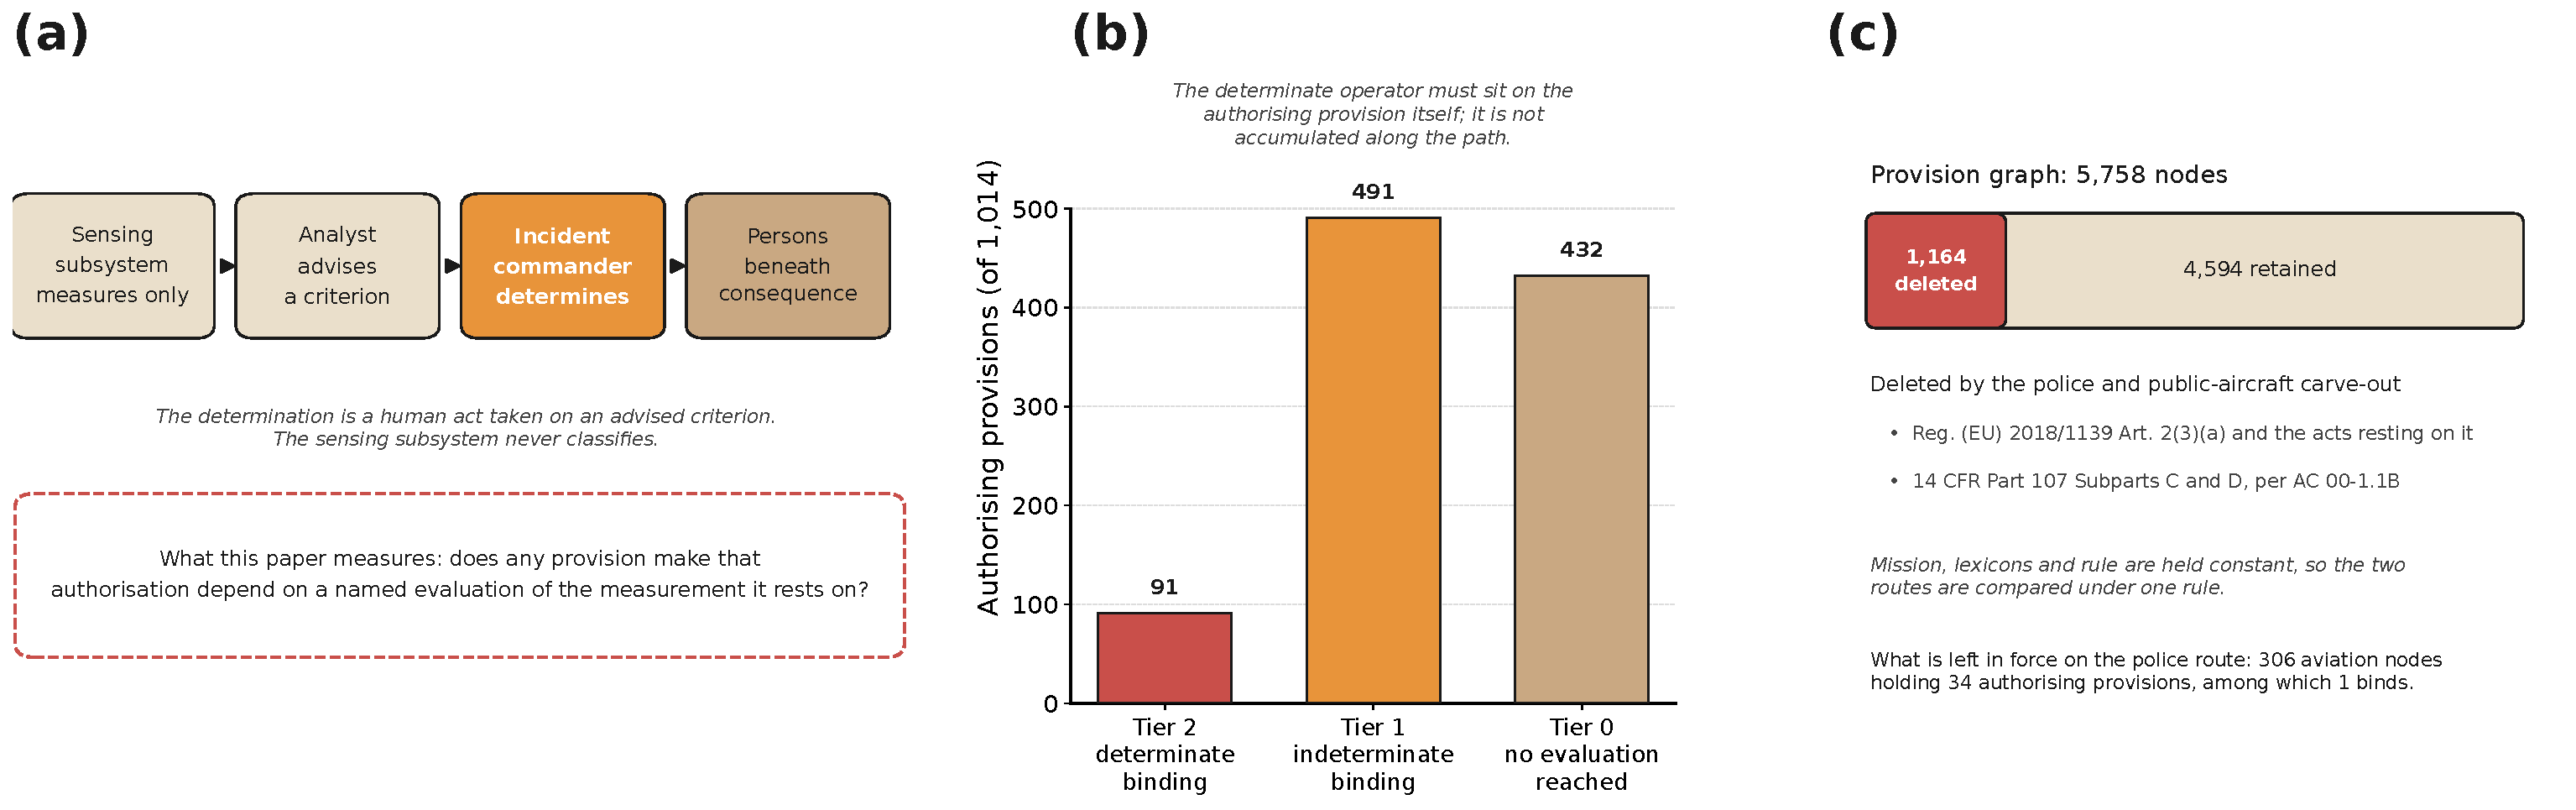
\includegraphics[width=\textwidth]{FigC}
\caption{What is measured. (a) In the ground mission, measurement, analysis and determination are separated by doctrine: the sensing subsystem never classifies, and the determination is a human act taken on an advised criterion. The question this paper measures is whether any provision makes the commander's authorisation depend on a named evaluation of the measurement it rests on. (b) The three tiers an authorising provision can occupy, with the corpus counts. The determinate operator must sit on the authorising provision itself; it is not accumulated along the path. (c) A police and public-aircraft carve-out is implemented as the deletion of nodes from the provision graph, so that the two routes are compared under one rule: Reg. (EU) 2018/1139 Art. 2(3)(a) and the acts resting on it, and 14 CFR Part 107 Subparts C and D per AC 00-1.1B; see Section 3.4 on why that set is conservative. Mission, lexicons and rule are held constant.}
\label{fig:f1}
\end{figure*}

\subsection{The provision graph}\label{sec:2.4}

Each instrument was decomposed to paragraph granularity: an article becomes a hub node carrying its heading, each numbered paragraph a node carrying its own text. Two qualifications on that sentence are owed, because an earlier version of this paper made it without them and it was not true as written. An article with no numbered paragraphs, which in the EU instruments is chiefly a definitions article, carries its numbered definitions instead, each as a node; a definitions article was previously held whole, so a seventeen-thousand-character article counted as one provision and fired on any term anywhere in it. And a United States section with a single unnumbered paragraph was, until the repair reported in Section 2.10, dropped entirely rather than kept as one node. Both are extraction defects and both are reported there with their measured effect. Annexes are cut from the article span and held separately, because EU annexes otherwise merge into the last article of the body. Each annex is held as a single node truncated at 6,000 characters, which is a severe limitation and we state its size: the retained fraction is 3.0\% of Directive 2014/32/EU's annexes, 5.3\% of Regulation 2018/1139's, 7.2\% of 2019/947's, 9.0\% of 2019/945's and 12.9\% of the AI Act's. The instrument-specific maximum permissible error tables of the metrology directive, the class requirements of 2019/945 and Annex III of the AI Act are therefore named in the corpus but not contained in it. A provision that refers to an annex can reach that node, and an evaluation term in the retained opening of an annex will ignite on it, but a condition written into an annex table below the cut cannot be read. Containment edges run downward only, from hub to paragraph and never between siblings, so that an operator in one paragraph is not read as governing its neighbours.

Reference edges were built by jurisdiction-specific grammars operating on paragraph text: EU internal and cross-instrument references; Korean internal references, cross-instrument references by quoted statute name, decree-to-parent-statute references, and the anaphor gateun beop (``the same Act'') resolved against the most recently named statute; Japanese references with kanji-numeral conversion; United States section references within and between Parts 107 and 89; and municipal and state-code internal references. A further two structural edge types were added: chapter and section hubs for the EU instruments, and edges linking a paragraph that says ``this Chapter'', ``this Section'', ``this Regulation'' or ``this Directive'' to the corresponding hub, since such phrases are references without a number.

The graph has 5,758 nodes and 8,834 edges: 4,296 containment, 374 chapter containment, 2,693 numbered internal references, 38 cross-instrument references, 959 unnumbered structural references, 187 decree-to-parent references, 184 annex references and 103 reverse-delegation edges.

\subsection{The predicate}\label{sec:2.5}

Three lexicons operate on node text. eval names a technical evaluation (certification, conformity assessment, test, inspection, audit, impact assessment, verification, accreditation, typeapproval, airworthiness, notified body, declaration of conformity, and Korean and Japanese equivalents). auth names an authorisation outcome (authorisation, permit, licence, registration, approval, placing on the market, eligibility, exemption, and equivalents). det marks determinate conditioning (``shall not . . . unless'', ``only if'', ``shall be revoked'', ``is required to'', and the Korean and Japanese forms that condition a permission on passing an examination), and nondet marks hedges (``should'', bare ``may'', ``as appropriate'', ``where necessary'', and equivalents).

The lexicons carry two exclusions, recorded here because each was introduced to remove a specific false positive. auth excludes activity verbs such as unhaeng and ts\={u}k\={o}; including them

made almost every Korean and Japanese traffic provision an authorisation. det is suppressed where the same unit says that a document must be included with, accompanied by or submitted with an application, because an attachment requirement is a filing formality rather than a condition on the outcome.

A provision is adjudicated as follows. If it carries auth, is not a penalty provision and is a paragraph rather than a hub, it is an authorising provision. From it, a breadth-first search of at most four hops looks for a node carrying eval. The determinate operator must be present on the authorising provision itself; it is not accumulated along the path. If any node on the path carries nondet, the path is capped.

\begin{itemize}
\item Tier 2, determinate binding: the provision carries a determinate operator and reaches a named evaluation within four hops with no hedge on the path.
\item Tier 1, indeterminate binding: the evaluation is reached, but the operator is absent or hedged.
\item Tier 0: no evaluation is reached.
\end{itemize}

The three tiers and the carve-out operation are set out in Fig. 1b and c.

The requirement that the operator sit on the start node is the correction of an error we made. An earlier implementation accumulated it along the path, so a start node with no operator could inherit one four hops away; back-tracing three implausible results exposed it. The uncorrected rule produced a far more striking headline than the corrected one supports, and we state both.

The four-hop bound is not arbitrary. Table 2 reports tier counts as the bound is relaxed. Tier-2 counts saturate: the fifth hop adds 1 return in the whole corpus, and removing the unnumbered structural and chapter edges entirely changes the count by 2.

\begin{table}[!htb]
\centering
\caption{Saturation of the path bound. All conditions use the same 1,014 authorising provisions.}
\label{tab:t2}
\small
\begin{tabular}{@{}lrrr@{}}
\toprule
Condition & Tier 2 & Tier 1 & Tier 0 \\
\midrule
No edges (provision read in isolation) & 72 & 283 & 659 \\
hop $\le$ 1 & 76 & 346 & 592 \\
hop $\le$ 2 & 88 & 442 & 484 \\
hop $\le$ 3 & 90 & 455 & 469 \\
hop $\le$ 4 (adopted) & 91 & 491 & 432 \\
hop $\le$ 5 & 92 & 495 & 427 \\
hop $\le$ 4, structural edges removed & 89 & 489 & 436 \\
\bottomrule
\end{tabular}
\end{table}

\subsection{Validating the lexicon}\label{sec:2.6}

The predicate is only as good as the vocabulary that feeds it, so the vocabulary was tested rather than asserted. The population at risk is tier 1: provisions that authorise and reach an evaluation but were scored as lacking a determinate operator. If the lexicon is leaky, the leak is there.

A sample of 36 tier-1 provisions was drawn with a fixed seed, stratified by language at 12 each for English, Korean and Japanese, and each was read and labelled for whether it does in fact condition an authorisation determinately on a named evaluation. Two of the 36 have since left the authorising population and are excluded. One left under the supplementary-provision repair

described in Section 2.3, having been recorded by the labeller as a transitional provision and not as a false negative. The other, Article 104-2-4(4) of the Japanese Road Traffic Act, was moved into the returned set by the lexicon symmetrisation of Section 2.10 and is therefore no longer in the population at risk; the labeller had recorded it as correctly scored, so its departure does not remove a false negative either. The sample is 34: 12 English, 12 Korean, 10 Japanese. Four were false negatives: 2 of 12 in English, 1 of 12 in Korean, 1 of 10 in Japanese. Allocation was equal across the three strata but the strata are not: the tier-1 population holds 222 English, 120 Korean and 149 Japanese provisions, so a pooled rate that ignores the weights understates the English stratum, which is the one with the highest observed rate. The design-consistent estimate is therefore the stratum-weighted one, 12.6\% with a 95\% interval of [4.7, 29.5] on the logit scale, projecting to 62 missed bindings across the 491 tier-1 provisions with an interval of 23 to 145. The unweighted pooled rate is 11.8\% [4.7, 26.6]; earlier versions of this paper reported that figure, and the weighted estimate replaces it because the sample was stratified and the weights are known.

Two features of this sample bear on that interval and were not stated until a reviewer asked for them. The first is that the sample is clustered by instrument in the same way the corpus is, which is the thing Section 3.3 corrects for elsewhere and did not correct for here. The 12 English provisions come from 6 instruments and both false negatives fall in one of them, the AI Act. The 12 Korean provisions come from 4. The 10 Japanese provisions come from one, the Road Traffic Act, so within that stratum there is no second cluster and the between-instrument component cannot be estimated at all. Treating instruments as sampling units within strata and using t(8) for the 3 strata and 11 instruments widens the interval from [4.7, 29.5] to [2.5, 45.0] per cent, a standard error of 0.083 against the 0.060 the provision-level calculation gives. Dropping the AI Act from the sample moves the weighted rate from 12.6 to 5.1 per cent and the projection from 62 to 25. Both intervals are reported in \texttt{verify/lex\\texttt{\_cluster}.json.} We report the narrower one as the headline because it is the one the stratification was designed for, and we carry the wider one beside it wherever the rate bears weight.

Neither interval is well identified, and the reason is worth stating because it bounds what any single number here can mean. The eight degrees of freedom are the design's, not the data's: one instrument, the AI Act, supplies 69 per cent of the variance, because it is the only sampled instrument in which a false negative occurred more than once. Accounting for that with a Satterthwaite correction gives 6.3 effective degrees of freedom on a per-stratum accounting and 2.0 on a per-instrument one, and the interval runs [2.3, 47.2] or [0.6, 78.2] per cent accordingly. A sample of 34 provisions with four false negatives across 11 instruments does not identify a rate to better than an order of magnitude, which is what this section said at the outset and what the corrected intervals now make arithmetic rather than rhetorical.

The second is that the sample was drawn from a tier-1 population of 480 provisions and the weights are computed on the current population of 491. 16 provisions entered tier 1 between those two states and all 16 are in the Japanese Road Traffic Act, which is 10.7 per cent of the Japanese stratum and had probability zero of being sampled; 5 left, and the two that were in the sample are the two reported above. Calling the estimator design-consistent puts weight on the frame, and the frame is not the population the estimate is about. Re-drawing the sample on the current population would close this and we have not done it.

On interpretation, two points bear. The rate is not higher in the non-English material, which is the asymmetry one would expect if the lexicon were an English instrument applied abroad. And none of the four concerns the sensing or measurement performance of a robot: they are a product conformity assessment on modification, a fundamental-rights impact assessment, a

driver aptitude test and a driving skill test.

Validation found two lexicon defects, and both were repaired before the reported run. The Korean authorisation pattern used a word boundary after the noun, and a word boundary does not occur between two Hangul syllables, so a licence followed directly by a particle did not match. The Korean and Japanese determinacy lists lacked the constructions that condition a permission on passing an examination, which meant the instrument missed Article 85(1) of the Korean Road Traffic Act and Article 89(1) of the Japanese Road Traffic Act, two of the most obvious determinate bindings in the corpus. The Korean construction was added at this stage; the Japanese one was not reached until the lexicon symmetrisation reported in Section 2.10, and Article 89(1) is one of the four Japanese bindings that repair produced.

The labels were applied in a single pass by the same investigator, reading each provision directly rather than through a language model, with no second pass and no second reader. The rate is therefore best read as an order-of-magnitude bound rather than a point estimate, and it is the one place in this paper where a reported figure rests on a single unreplicated reading. The projection it carries into Figure 4c should be read with that in mind.

\subsection{Auditing the bindings}\label{sec:2.7}

The lexicon validation above measures how often the predicate misses a binding. It says nothing about how often what it returns is not one, and that is the population every number in this paper is computed over. We therefore audited it in full rather than by sample.

Each of the 91 provisions the predicate returned was prepared as an audit record containing the provision text, every lexicon pattern that fired on it with the string actually matched and eighty-five characters of surrounding context, the path the predicate recorded, and the node at which an evaluation term ignited. Seventy-three of the 91 were available when the two-pass labelling was carried out. The other 18 entered the returned set afterwards, under corrections reported in Section 2.10: 3 under the operator correction, 5 under the extraction repairs, and 10 under the lexicon symmetrisation. Each of the 18 was prepared as a record in the same form and adjudicated under the same three conditions, by the same procedure but once rather than twice, and the adjudication of each is released with the labels. Every agreement statistic in this section is therefore computed on the 74 records the two passes saw, of which 73 remain in the current returned set, and not on the 91, and a reader who wants the agreement figure for the whole returned set will not find it here, because it was not measured. The 73 records were labelled twice, in two passes carried out by the same investigator using a large language model as the labelling instrument, the second pass made without sight of the first pass's labels and with the records presented in a different order. This is a consistency check on the labelling procedure under repetition, not an inter-rater reliability measurement between two people, and the agreement statistics below should be read only as the former. Both passes applied three conditions derived from the construct itself. A provision is a binding only if (i) it confers or conditions a legal permission, rather than mentioning another regime's permission, defining a term, prohibiting a false mark, deeming a prior authorisation, or listing the documents an application must carry; (ii) the determinate operator conditions that permission, rather than governing a different clause that the pattern window happened to span; and (iii) the object of that condition is a named evaluation procedure, rather than an evaluation term appearing as a date reference, as an item in a definition list, as a section heading, or as the authorisation the provision itself issues.

Labels were recorded on three values, not two: binding, not a binding, and borderline, the third reserved for a record a pass could not place under the conditions as written. The marginals differ between the passes, 43 / 27 / 4 in the first and 26 / 47 / 1 in the second, and the full

\begin{figure*}[!t]
\centering
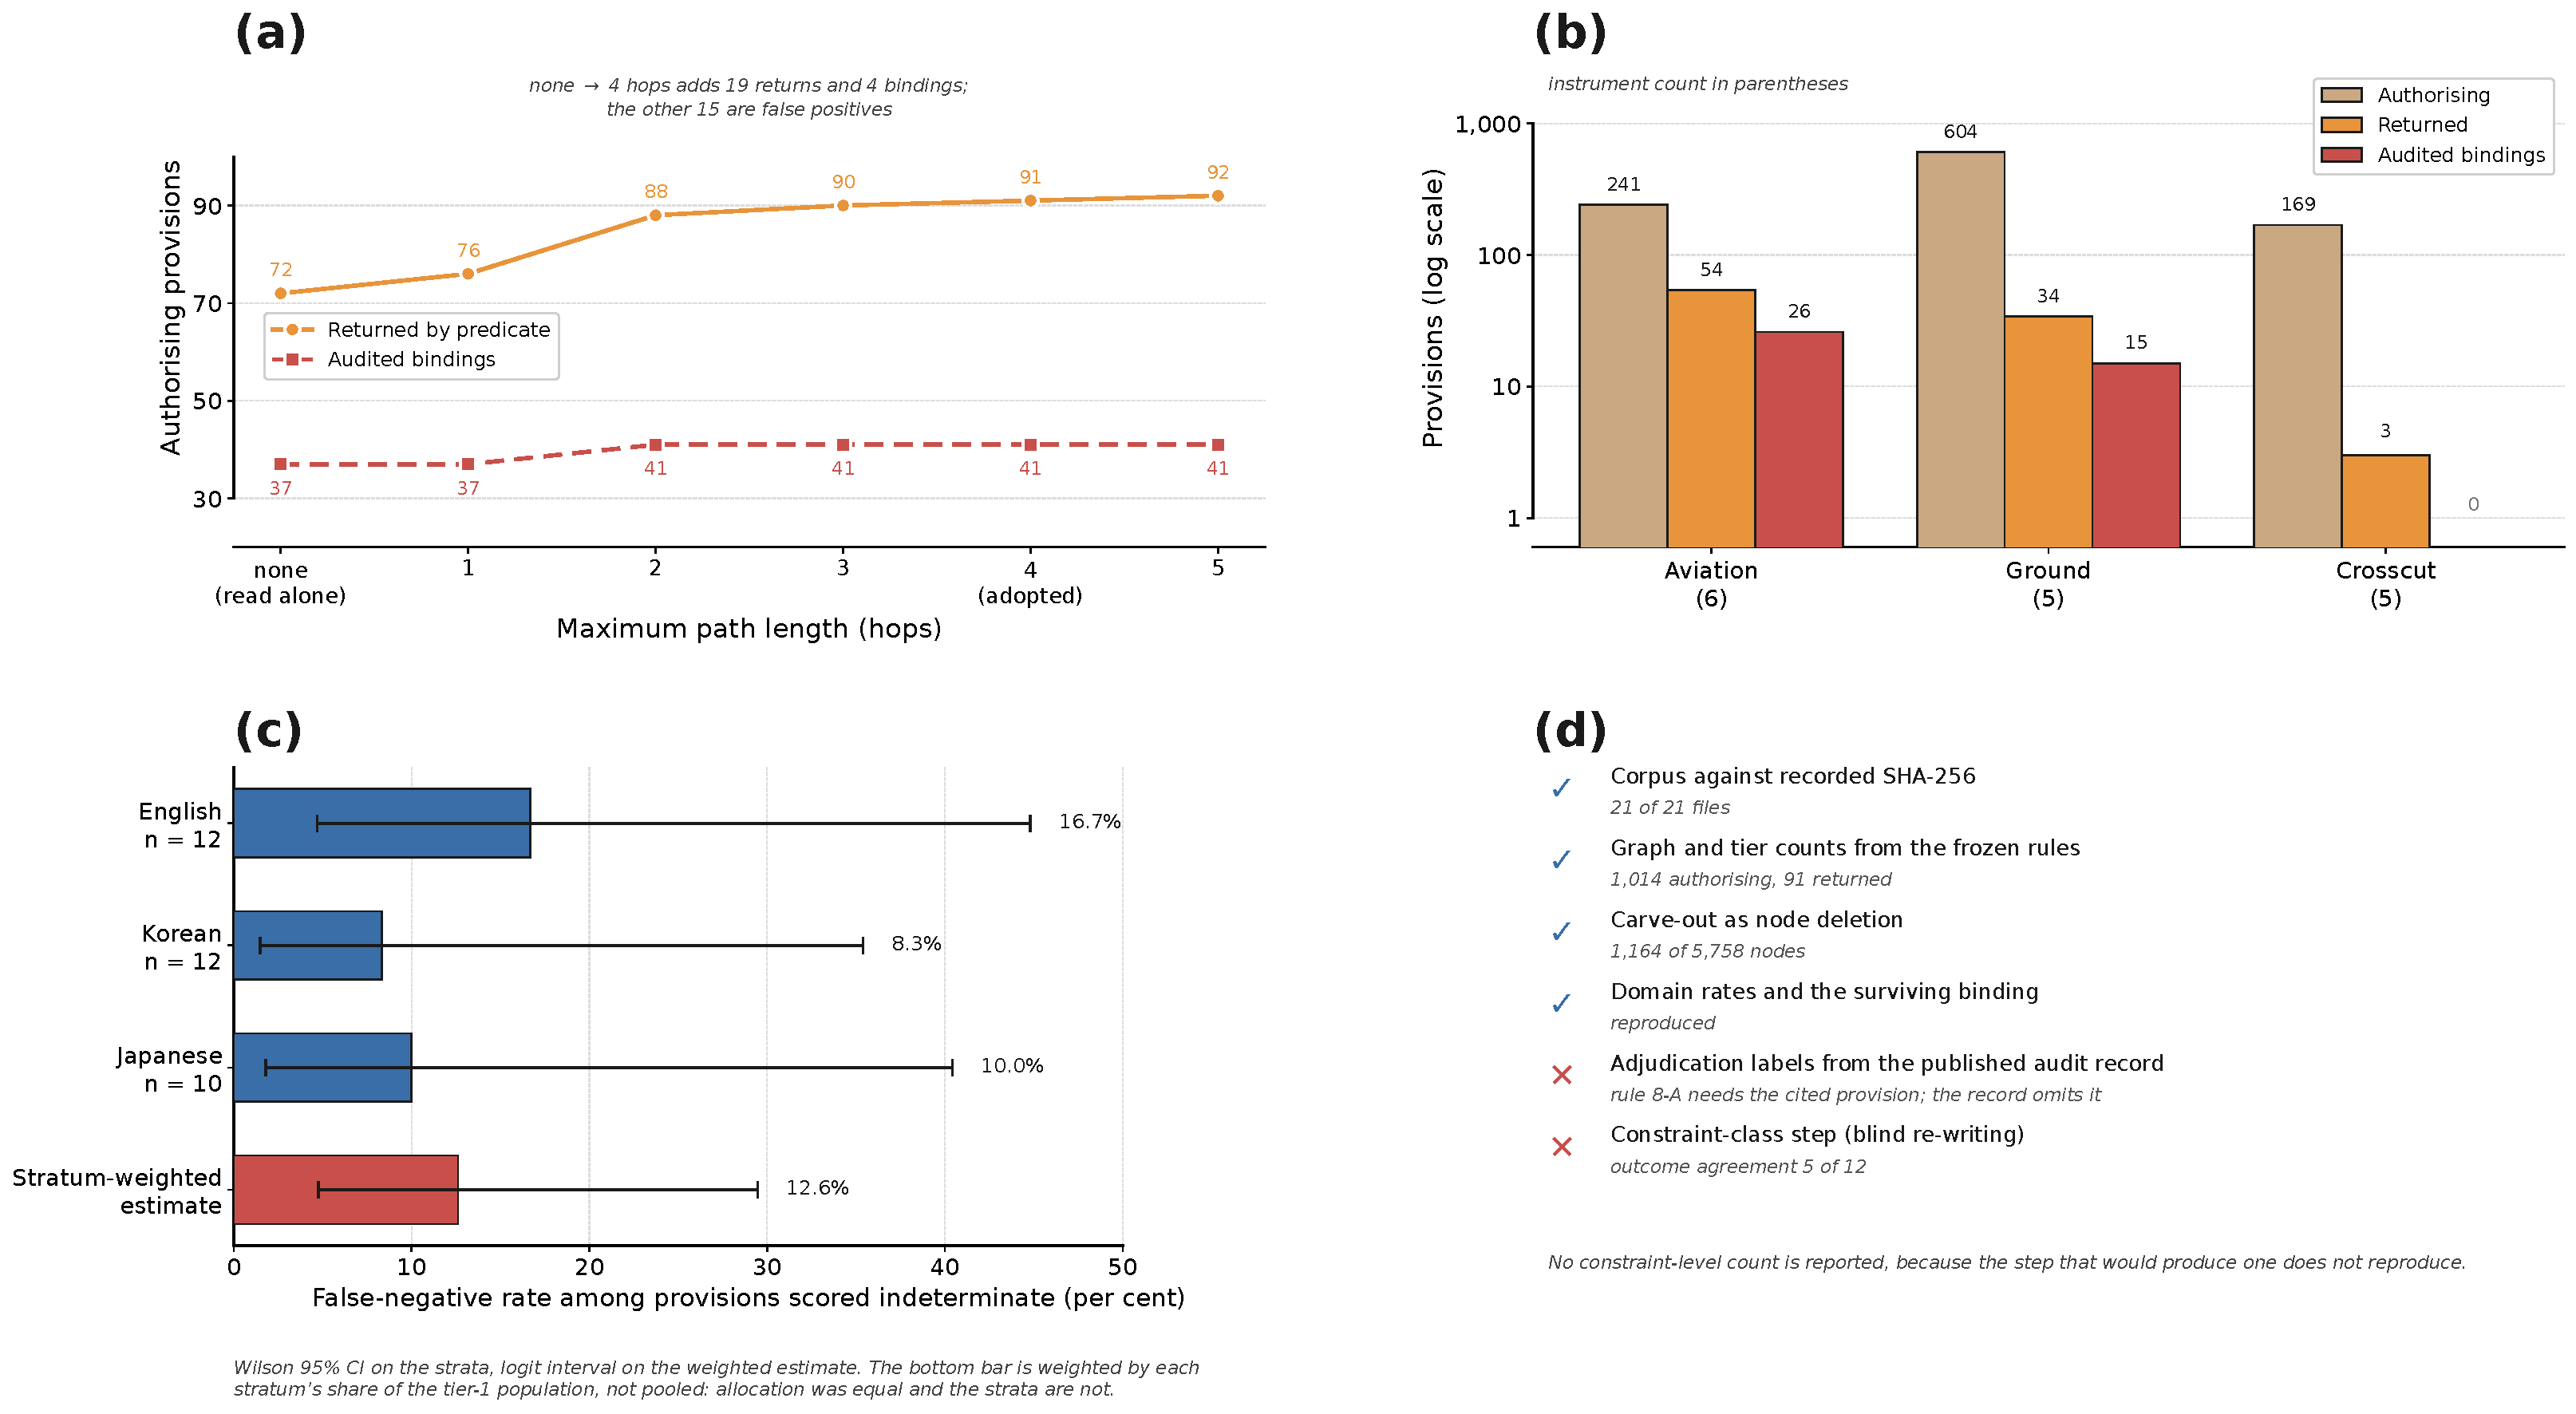
\includegraphics[width=\textwidth]{FigM}
\caption{Checks on the measurement. (a) Provisions the predicate returns and provisions the audit confirms as bindings, both as a function of the maximum path length. Going from a single-provision reading to four hops adds 19 returns and 4 bindings, so the 15 remaining additions are false positives and following cross-references lowers precision from 0.514 to 0.451 (Table 7). (b) Composition of the audited corpus by regulatory domain, with the number of instruments in each. (c) Lexicon validation: the false-negative rate among provisions scored indeterminate, by language, with Wilson 95\% intervals on the strata and a logit interval on the weighted estimate. The plotted interval is the design-consistent one; treating instruments as sampling units within strata widens it to [2.5, 45.0] per cent (Section 2.6). The Japanese stratum is n = 10 because one sampled provision left the authorising population under the repair of Section 2.3 and a second under the symmetrisation of Section 2.10. The bottom bar is the stratum-weighted estimate, not a pooled one: allocation was equal and the strata are not. (d) What reproduces and what does not. The constraint-level step does not, which is why no constraint-level count is reported.}
\label{fig:f2}
\end{figure*}

cross-tabulation is released with the labels, because the three-valued scale is what the agreement statistics below are computed on and a reader who assumes two values will not reproduce them. Agreement between the two passes was 51 of 74, Cohen's $\kappa$ = 0.448. That figure should not be read on the conventional scale, because the two passes have different marginals: 43 / 27 / 4 against 26 / 47 / 1 is a bias index of 0.23, and with those marginals fixed the largest agreement arithmetic allows is 54 of 74, so $\kappa$max = 0.520. The observed $\kappa$ is 86 per cent of its own ceiling. Gwet's AC1, which does not inherit the marginal bias, is 0.577. What the three numbers say together is not that the labelling was moderately reliable but that it was close to as consistent as a systematic shift in threshold between the passes permits. That shift is our own doing: the second pass received an interpretation directive on condition (iii) that the first did not, so the two passes were not given identical instructions, which is why we report agreement both over all 74 labelled records and over the subset that directive does not concern. Eighteen of the twentythree disagreements fall on one sentence pattern, used throughout Regulation (EU) 2018/1139, in which a certificate shall be issued upon application, when the applicant has demonstrated that it complies with the implementing acts of a named article. Restricting to the 56 provisions outside that pattern, agreement is 51 of 56 and $\kappa$ = 0.835. That number estimates nothing. It is obtained by deleting the single cell that holds eighteen of the twenty-three disagreements, so it describes the residue after the disputed pattern is removed and is reported only to locate the disagreement, not to quantify reliability. The disagreement is therefore not instability in the labelling but an ambiguity in condition (iii) that we had not resolved in advance, and we resolve it here, in the direction that excludes: a sentence of that form names no evaluation procedure. The term it offers is either the certificate it is itself issuing, which cannot be its own condition, or the bare verb demonstrated that, which is not a procedure. All eighteen are counted as false positives, as are the three remaining disagreements in which an evaluation term appears only as a descriptor of who is examined or when; the two in which the operator's object is a named examination are counted as bindings.

Forty-one of the 91 provisions are bindings. Precision is 0.451. It is not uniform: 26 of 54 in aviation (0.481), 15 of 34 on the ground (0.441), and 0 of 3 among the cross-cutting instruments (0.000).

The interval on that figure needs saying carefully, because 41 of 91 is a census of the returned set and not a sample from it. The Wilson 95\% interval of [0.352, 0.553] is the interval that would apply if these 91 provisions were a random draw from a larger population of returns. They are not: they are all of them, drawn from sixteen purposively selected instruments, two of which were added late precisely because they were the most likely to refute the paper, and Regulation (EU) 2018/1139 alone supplies 32 of the 91 returns and 17 of the 41 bindings. Resampling the eleven instruments that contribute returns with replacement, 10,000 draws at a fixed seed, and recomputing the precision in each draw, gives [0.306, 0.518], which is a quarter wider and is the interval to use for any statement about how this predicate would behave on instruments other than these sixteen. What that interval generalises over is instruments drawn like these, which is a hypothetical population rather than an observed one, and with eleven clusters it is coarse: the resampled precision takes a limited number of distinct values and the quantiles inherit that discreteness. We report both, and where this paper says that a returned count is an upper bound on bindings, the claim rests on the census point estimate and needs neither interval. Every count this paper reports is therefore given twice, as the number of provisions the frozen predicate returns and as the number that survive the audit, and the second is the one the argument rests on.

This audit establishes the numerator. It says nothing about the denominator, and the denominator was audited separately and found to be contaminated at a comparable rate; Section 2.8

reports that audit and the corrected rates it implies.

The audit names the false positives by mechanism, and one of those mechanisms deserves a paragraph because the obvious repair does not work. The determinate-operator patterns scan a window of up to 200 characters, and the window steps over negation. Article 5(5) of Regulation (EU) 2019/947 says that a UAS operator who has filed a declaration for a standard scenario shall not be required to obtain an operational authorisation, which is an exemption, and the predicate records it as a binding. Nine of the 1,014 authorising provisions carry a determinate pattern inside a negated context and four of those reach tier 2. The repair that suggests itself is to suppress a determinate operator whose match lies within a negated clause. We implemented it and did not adopt it, because it removes a binding as well. Article 5(1) of the same Regulation reads where one of the requirements laid down in Article 4 or in Part A of the Annex is not met, a UAS operator shall be required to obtain an operational authorisation, where the negation governs the condition and the operator is affirmative; a proximity rule cannot tell the two apart, and the paragraph it deletes is the one audited binding that exists only because a cross-reference is followed (Section 3.2). Applied to the corpus the guard returns 88 provisions instead of 91, drops two false positives and one binding, and leaves precision near unchanged at 0.455. Three of the four negated tier-2 provisions fall; the fourth, Article 16(1) of Regulation (EU) 2018/1139, carries a second determinate match outside any negated context and so survives a guard that acts on matches rather than on provisions. Separating the two cases needs the operator's clause boundary rather than a character window, which is the same limit that produces the other mechanisms in this list, so we report the defect and leave the rule alone.

The resolution of condition (iii) was made after the labels were seen, which makes it the one rule in this paper that could have been chosen to suit the answer, so we report what the other choice would have given. Resolving in the direction that includes revives 12 of the records the adjudication rejects and gives 53 bindings instead of 41, a precision of 0.582 instead of 0.451. Every headline survives that change and two of them strengthen: the police carve-out leaves exactly one audited binding in force in either direction (38 to 1 instead of 26 to 1), the cross-cutting instruments still produce none, and the aviation-to-ground ratio rises from 4.34 to 6.35 with Cohen's h from 0.353 to 0.500. We adopt the excluding direction because it is the conservative one on the construct and because it is the direction that makes our own headline weaker, and we report the other so that a reader can see the choice did not manufacture the result (Table 3).

\begin{table}[!htb]
\centering
\caption{Both resolutions of the ambiguity in condition (iii). The adopted direction is the one that yields the smaller count.}
\label{tab:t3}
\small
\begin{tabular}{@{}lrrrrrr@{}}
\toprule
Resolution & Bindings & Precision & Aviation & Ground & Cross-cut & Carve-out \\
\midrule
Excludes (adopted) & 41 & 0.451 & 26/241 & 15/604 & 0/169 & 26 $\rightarrow$ 1 \\
Includes (alternative) & 53 & 0.582 & 38/241 & 15/604 & 0/169 & 38 $\rightarrow$ 1 \\
\bottomrule
\end{tabular}
\end{table}

The audit was performed after the ruleset was frozen and the predicate had been run, and the frozen ruleset was not changed in response to it. Tuning the lexicon or the path bound against these labels would convert a measurement into a fit. The labels, the audit records and the adjudication rule are released with the other materials.

The labels this paper adopts are not the labels its first release reported, and the difference is large enough to state here rather than in a limitation. The two passes described above resolved to 34 bindings, and that is the count the earlier version published. The audit records released with it carried every lexicon match and the path the predicate recorded, but not the text of the provision a path arrived at, so the rule that admits a binding reached through a named provision could not be applied from the record alone; a reader working from the released records could not reproduce the adjudication. We enriched the records with the cited text and had the audit repeated, blind, against a rubric from which the counts had been removed. That pass moves 10 of the 91 records and gives 41. On the binding value the three passes stand at 43, 26 and 41, so the labelling is not stable to the procedure that produces it, and the adopted count is the third pass rather than an average of them. What the change does not move is the comparison the paper rests on: Cohen's h goes from 0.357 to 0.353 and the aviation-against-ground Fisher test from p = 1.5 $\times$ 10$-$6 to p = 2.6 $\times$ 10$-$6 . The direction of the change is against us in the headline rate, which rises from 3.4 to 4.0 per cent, and in favour of us in the precision, which rises from 0.374 to 0.451. All three label sets are released.

\subsection{Auditing the denominator}\label{sec:2.8}

The audit of Section 2.7 establishes that 41 of the 91 provisions the predicate returns are bindings. It leaves the denominator unexamined, and a rate is two numbers. If the authorising population is itself contaminated, every rate in this paper is understated by whatever the contamination is, and the understatement need not be uniform across domains. Reporting a well-audited numerator over an unaudited denominator would be the same error we criticise in the coding literature, one level down.

We therefore audited the denominator by the same procedure. Eighty authorising provisions were drawn with a fixed seed and prepared as records carrying the provision text and the authorisation pattern that fired, with no tier information and no indication of whether the predicate had returned the provision. Each record was labelled against the definition this paper states in Section 2.1: a paragraph of a legal instrument that grants, conditions or withdraws a permission, and is not a penalty provision. As with the binding audit, the records were labelled twice, the second pass in reverse order and without sight of the first. Agreement was 76 of 80. One of the eighty, 14 CFR \S{}89.515, has since left the authorising population under the paragraph-node repair of Section 2.10; the labeller had recorded it as not an authorising provision, so its departure removes a record from the denominator without removing a positive, and the precision below is computed on the 79 that remain. The four disagreements were adjudicated against the provision text: Article 71-5(1) of the Japanese Road Traffic Act, which bars driving without a displayed novice mark, was included because its form is the one this paper counts elsewhere, and three were excluded as procedural duties to issue or record a document, or as a prohibition on using a similar trade name.

Thirty-nine of the 79 remaining sampled provisions authorise: a denominator precision of 0.494 with a Wilson 95\% interval of [0.386, 0.602], projecting the authorising population to 501 provisions with an interval of 392 to 610. The contamination is not uniform, but the pattern is not the one an earlier draw suggested. It is lightest on the ground, where 22 of 40 sampled provisions authorise, and heaviest among the cross-cutting instruments, where 5 of 15 do; aviation falls between at 12 of 24. A first draw, made on the pre-repair population of 1,003, put aviation at 4 of 17 and the pooled precision at 0.375; the two Wilson intervals overlap, but the aviation cell in that draw held four events and we report the second draw rather than the first, because the first was taken over a population two extraction defects have since changed.

The dominant mechanism is institutional and procedural rather than lexical. Of the 41 sampled provisions the audit excludes, the largest groups are duties on an authority or a body to notify, consult, record, verify or issue a document, and provisions allocating tasks, establishing procedures or empowering the Commission to adopt acts. All nine exclusions in the Korean enforcement rule are of this kind, as are six of the nine in Regulation (EU) 2018/1139. Definitions account for three. An earlier draft attributed the contamination chiefly to recitals, definitions and annex headings in the aviation material; that description does not survive the second draw and we withdraw it.

No sampled provision was a penalty provision. The first draw found three that the exclusion patterns missed, all in the Korean and Japanese material; the United States patterns added in Section 2.10 and the second draw together give no further instance, which is evidence that the exclusion now executes, not proof that it is complete.

Table 4 gives the nominal and corrected rates. Correcting the denominator raises the aviation rate from 10.8\% to 21.7\% and the ground rate from 2.5\% to 4.5\%, and because the correction is larger in aviation it widens rather than narrows the contrast the paper rests on: the aviationto-ground ratio goes from 4.3 to 4.8. The corrected rates carry the interval of the denominator

audit, and Table 4 reports them with it; the numerator contributes no interval because the audited binding count is a census of the returned set rather than a sample from it, and an earlier version of this sentence claimed a numerator interval the released script does not compute; the aviation interval runs from 13.9 to 30.4 per cent on a cell of 24 sampled provisions, which is wide enough that we treat the nominal rates as the statement the paper rests on and the corrected rates as a check on their direction. Two further cautions belong with them. The estimator multiplies a nominal count by a sampled precision, so it inherits the upward bias of a plug-in ratio at small cell sizes. And the two draws we have made returned pooled precisions of 0.375 and 0.494; those intervals overlap, but a single point estimate is not a stable basis for correcting a whole population, which is the second reason the nominal pair carries the argument. No conclusion in this paper depends on which pair is used.

\begin{table}[!htb]
\centering
\caption{Binding rates before and after correcting the denominator for the contamination measured in Section 2.8. ``Auth.'' is the nominal authorising count; ``Corr.'' is that count multiplied by the audited precision of the denominator in that domain, and the interval on the corrected rate carries the Wilson interval of that precision. The audited binding count is the same in both columns, because the binding audit's condition (i) applies the same test as the denominator definition, so a provision counted as a binding is by construction inside the true authorising set. The corrected figures rest on domain cells of 24, 40 and 15 sampled provisions and should be read with that in mind; the plug-in estimator B/(N $\hat{p}$) is also upward-biased at these cell sizes. The Wilson intervals in this table are computed on provisions and carry no correction for the instrument clustering that Section 3.3 measures; the corrected intervals of Table 9 are the ones that carry it. The corrected authorising counts do not add: the three domain cells sum to 508 against the 501 in the Total row, because the plug-in estimator is applied to each cell's own audited precision and is not additive across cells.}
\label{tab:t4}
\small
\begin{tabular}{@{}lrrrrrr@{}}
\toprule
Domain & Bindings & Auth. & Nominal & Denom. prec. & Corr. auth. & Corrected rate \\
\midrule
Aviation & 26 & 241 & 10.8\% & 12/24 = 0.500 & 120 & 21.7\% [15.7, 34.3] \\
Ground & 15 & 604 & 2.5\% & 22/40 = 0.550 & 332 & 4.5\% [3.6, 6.2] \\
Cross-cut & 0 & 169 & 0.0\% & 5/15 = 0.333 & 56 & 0.0\% \\
Total & 41 & 1,014 & 4.0\% & 39/79 = 0.494 & 501 & 8.2\% [6.7, 10.5] \\
\bottomrule
\end{tabular}
\end{table}

\subsection{The carve-out as node deletion}\label{sec:2.9}

Mission A can be flown on two routes. The civil route is adjudicated against the full corpus; the police route against the same corpus with the provisions that do not apply to police operations deleted from the graph. Everything else is held constant, so the difference between the two is a measurement rather than an argument.

Deletion is driven by two documented carve-outs. Regulation (EU) 2018/1139 Article 2(3)(a) provides that the Regulation does not apply to aircraft, and equipment to control aircraft remotely, while carrying out military, customs, police and similar activities or services under the control and responsibility of a Member State, undertaken in the public interest by or on behalf of a body vested with the powers of a public authority, together with the personnel and organisations involved; Regulations (EU) 2019/947 and 2019/945 rest on that basic act and are deleted with it.

Three features of that provision bear on what the deletion models, and we state them because the first two narrow it and the third is the reason the comparison is worth making at all. The exclusion is indexed to an activity rather than to an airframe: while carrying out means that the same unmanned aircraft is inside the Regulation on Monday and outside it on Tuesday, according to what it is doing. The deletion therefore models a specific condition, a police mission flown under the control and responsibility of a Member State by a body vested with public-authority powers, and not a standing status that attaches to police equipment. It also carries conditions of

its own that a real agency would have to satisfy, and an operation failing any of them stays inside the Regulation.

The third is that the exclusion is not a void. The second subparagraph of Article 2(3) provides that Member States shall ensure that the activities and services performed by those aircraft are carried out with due regard to the safety objectives of this Regulation, and that where appropriate those aircraft are safely separated from other aircraft. That is the whole of what survives the carve-out on the European side, and its two operative standards are due regard and where appropriate, both of which this paper's own hedge lexicon matches. The provision that replaces a certification regime for police flight is, on the predicate's own reading, indeterminate. We report this as a legal reading of the carve-out rather than as a measurement, because Article 2(3) is a scope provision and the audited population is drawn from authorising provisions; the predicate does return it, at tier 1. FAA AC 00-1.1B paragraph 12 states that other civil certification and safety oversight regulations do not apply to public aircraft operations, and that a public aircraft operator may self-certify standards for unmanned aircraft airworthiness as well as pilot certification, qualification and medical standards; 14 CFR Part 107 Subpart C and Subpart D are deleted accordingly.

This removes 1,164 of 5,758 nodes: 682 from Regulation 2018/1139, 232 from 2019/945, 133 from 2019/947, 68 from Part 107 Subpart C and 49 from Subpart D. Subparts A, B and E of Part 107 are retained, as is the whole of Part 89, which is not among the provisions AC 00-1.1B exempts. Every borderline case was resolved in favour of retention, which is the direction that makes the police route look better covered than it is.

Deleting Regulation 2019/945 needs its own justification, because that Regulation imposes duties on a manufacturer placing a product on the market rather than on the operator who later flies it, and an operator-side exemption does not obviously reach it. The justification is in its own scope provision. Article 2(1) states that Chapter II applies to UAS intended to be operated under the rules and conditions applicable to the `open' category of UAS operations or to operational declarations under the `specific' category of UAS operations pursuant to Regulation (EU) 2019/947. The class-marking regime is therefore indexed to operation under 2019/947, which is the regime the police route does not enter. We none the less report what happens if the objection is granted, because the answer does not depend on resolving it: retaining the whole of Regulation 2019/945 on the police route raises the returned count from 7 to 8 and leaves the audited count at 1, the same surviving binding. Regulation 2019/945 contributes no audited binding on either route, so its treatment cannot change the result (Table 5).

The second variant is the one that does change it. Article 2(6) of Regulation 2018/1139 allows a Member State to decide to apply parts of Chapter III to the activities excluded by Article 2(3)(a). No such decision is modelled in the adopted deletion, which is why the Limitations call the carveout elective rather than automatic. Restoring the whole of Regulation 2018/1139 puts 18 audited bindings back in force on the police route, 17 of the 25 audited bindings the carve-out removes. We previously called this an upper bound on what such a decision could return; it is not one. Section VII of Chapter III is Unmanned aircraft, and Implementing Regulation 2019/947 and Delegated Regulation 2019/945 are adopted under it, so a Member State decision applying that Section would plausibly carry those acts with it, and this row restores only the basic act. It is a partial restoration and the figure is a lower bound on what the decision could return, not an upper one.

\begin{table}[!htb]
\centering
\caption{The police route under three deletion sets. The adopted set is the first row. The second grants the objection that the product regime is not operator-indexed; the third is a lower bound on a Member State decision under Article 2(6).}
\label{tab:t5}
\footnotesize
\begin{tabularx}{\textwidth}{@{}Xrrr@{}}
\toprule
Deletion set & Nodes retained & Returned & Audited \\
\midrule
Adopted & 4,594 & 7 & 1 \\
Regulation 2019/945 retained & 4,826 & 8 & 1 \\
and 2018/1139 also restored (Art. 2(6), partial) & 5,508 & 40 & 18 \\
\bottomrule
\end{tabularx}
\end{table}

\subsection{Freezing and falsification}\label{sec:2.10}

Seventy-nine files are frozen: the corpus manifest and the provision graph, the lexicons, the node extractor, the reference grammars, the structural-edge builder, the path and tier logic, the scope restriction, the carve-out rule, the adjudication executor and its label register, the three label files, every script that writes an output this paper cites, the script that assembles this manuscript from its parts, and the four figure scripts with the eight image files they produce, and the script that measures how saturated the evidence vocabulary is. The files are hashed individually and the concatenation of their hashes is hashed again. The count in the preceding sentence is the one \texttt{verify/seal\\texttt{\_audit}.py} prints, and a released check fails if the two differ; an earlier version stated forty-five while the register held forty-seven, in the same paragraph that had just assigned the count to the script.

An earlier version of this sentence said that every file which can influence an outcome was frozen, and a reviewer established that it was not true. The scope restriction, which is the sole source of the domain partition and whose admissibility test the frozen adjudication executor imports, was outside the seal, as was the adjudication label register that produces the audited count itself. Ten modules present in the first freeze had been dropped without record by the time of the fourteenth, and twenty-five of the scripts that write cited outputs were never in it, one of them a script the freeze record itself names as affecting measurement. All are now inside. We no longer state the seal as exhaustive: a released script, \texttt{verify/seal\\texttt{\_audit}.py}, counts what it does not cover on every run and fails if any script that writes a cited output sits outside it, and the count it reports is the claim rather than our assertion.

Two further gaps in the apparatus were found after that and are closed here rather than disclosed. The first is that the apparatus sat outside the thing it audits: the script that computes the generation hash was not itself among the frozen files, so replacing its output with a constant left every gate passing. Eleven files of apparatus, the hash script and the four gates that read it among them, are now frozen with the rest. The three files that hold the consistency suite were outside the seal until this version, which mattered because a check can be replaced by a trivially true one without changing the number of checks the suite reports; those three are frozen as well, so a change to any of them moves the generation hash.

A third gap was of the same kind and was created by one of these repairs. The check that the figures in the manuscript are the ones the released figure scripts produce compared each figure against a record of hashes, and that record was written by the build script, which the gate runner invokes immediately before the check. The build script does not regenerate the figures; it copies them. So the record was always a record of whatever was on disk at that moment, and the check could not fail. We established the size of this by replacing one results figure with another of the paper's own figures: every gate and every check passed. The expected hashes now come from the freeze record, which only an explicit refreeze writes, and the figure scripts and their outputs are in the seal, so a substitution moves the generation hash as well. The same repair removed a

comment that claimed the assembled manuscript was checked by reassembling it and comparing bytes while the code compared hashes the build had just written; the assembly logic is now a separate released script and the check reassembles with it and compares bytes, which does not depend on what ran first.

That does not close the hole, and saying that it did would repeat the error. A reviewer put it back in three lines: replacing the hash function's output with a constant and then altering a frozen input still leaves every gate passing, because the hash that is supposed to detect the alteration is computed by a file the alteration can reach. Sealing the apparatus inside its own seal is circular. What actually caught the substitution was the consistency suite comparing each frozen file against the per-file digests recorded in the freeze record, and the freeze record is not in the seal. So the root of the guarantee is one file outside the thing it guarantees, and anyone who can write that file can write a consistent set. We state the position rather than a stronger one: the apparatus detects accident and drift, which is what it was built for and what it has repeatedly done, and it does not detect an author who edits both an input and the record of that input. The only fix is an external anchor, and the deposited archive's identifier is where the freeze record's hash is pinned beyond our reach; until that identifier exists, the chain is internal and we do not claim otherwise. The second is the provenance stamp each output carries. It was written afterwards by a separate pass that selected files by modification time, which could be reproduced with two shell commands and which, on the same frozen inputs, stamped a different set of files on each run. Each script now writes its own stamp at the moment it writes its output, and the stamping pass is retired. The stamp therefore records that this generation's code produced this output. It is not evidence that nothing was altered afterwards, because whoever can write the output can write the stamp, and we do not offer it as such. Two outputs were also exempt from the freshness gate on the stated ground that they were corpus facts independent of the ruleset. That ground was wrong, since the corpus manifest and the node extractor are both frozen, and while the exemption held, one of the two came to hold an annex length that the current corpus does not reproduce. Both are now regenerated and checked with the rest. The adjudication re-runs bit-identically across hash seeds, which required sorting the adjacency lists; an earlier version reported tier counts stably but recorded paths that varied between runs, and the claim of bit-identical reproduction was not true until this was fixed.

Ten changes have been made to the frozen files and rules since, and each is recorded with its measured effect rather than absorbed silently. Appendix A gives them in full, one paragraph each, with what prompted the change and what it moved. Table 6 gives the net effect of the set on the quantities this paper reports, so that a reader who wants to know whether the ruleset was tuned to the answer can see the direction of every move without reading the appendix. Three of the ten moved a headline figure against us, four moved one in our favour, and three left every reported quantity unchanged; the two largest in absolute terms are the lexicon symmetrisation, which added nine returned provisions and four audited bindings, and the paragraph test, which removed five authorising provisions from the aviation denominator and so raised the aviation rate.

Nothing else was altered: no path bound, hedge rule or scope restriction was changed in response to the audit, although the audit identifies several that would raise precision if changed. All ten are reported because a frozen ruleset is only worth freezing if departures from it are visible, and the hash chain of the current files is republished with the materials so that the versions can be compared.

The design states its own defeater, and the defeater was met. The claim an earlier version of this paper made was that outside aviation, and inside aviation outside the civil route, no provision

\begin{table}[!htb]
\centering
\caption{Net measured effect of the ten changes to the frozen files and rules. ``Before'' is the state at the first freeze that reported each quantity, and for the rows that depend on labels it is that state as labelled then, because the pre-change returned sets were not re-labelled under the adjudication this paper adopts; ``after'' is the current frozen run. Appendix A attributes each move to the change that produced it. Direction is relative to the claim this paper makes: a change that raises the predicate's precision, or lowers the rate at which bindings appear, makes the paper's negative claim easier to sustain and is marked favourable.}
\label{tab:t6}
\small
\begin{tabular}{@{}lrrr@{}}
\toprule
Quantity & Before & After & Direction \\
\midrule
Corpus nodes & 5,568 & 5,758 & neutral \\
Graph edges & 8,596 & 8,834 & neutral \\
Authorising provisions & 1,003 & 1,014 & neutral \\
Returned provisions & 77 & 91 & against \\
Audited bindings & 27 & 41 & against \\
Precision of the predicate & 0.351 & 0.451 & favourable \\
Aviation-to-ground ratio & 8.07 & 4.34 & against \\
Lexicon false-negative rate & 11.1\% & 12.6\% & against \\
Surviving binding on police route & 1 & 1 & unchanged \\
\bottomrule
\end{tabular}
\end{table}

conditions a determinate authorisation outcome on a named evaluation of a performance property of the machine; one provision that authorises, carries a determinate operator and reaches such an evaluation within four hops would refute it. Section 3.4 reports that provision. It is 14 CFR \S{}89.110(b), it survives the police carve-out, and it is the reason the claim this paper now makes is narrower and is stated in terms of what the evaluation is about. The surviving binding conditions operation on an accepted declaration that the aircraft reports its own position to a stated accuracy. It says nothing about the accuracy of anything the aircraft senses, and the corpus contains no provision in force on the police route that does. This is a weaker claim than the one we set out to test and it is the one the measurement supports. The corpus, graph, lexicons and executor are released so that the search can be run by anyone, including against instruments we did not include, and the defeater stands in the same form: one provision in force on the police route that conditions an authorisation on a named evaluation of sensing performance refutes it.
